% Created by tikzDevice version 0.12.3 on 2020-04-26 21:53:18
% !TEX encoding = UTF-8 Unicode
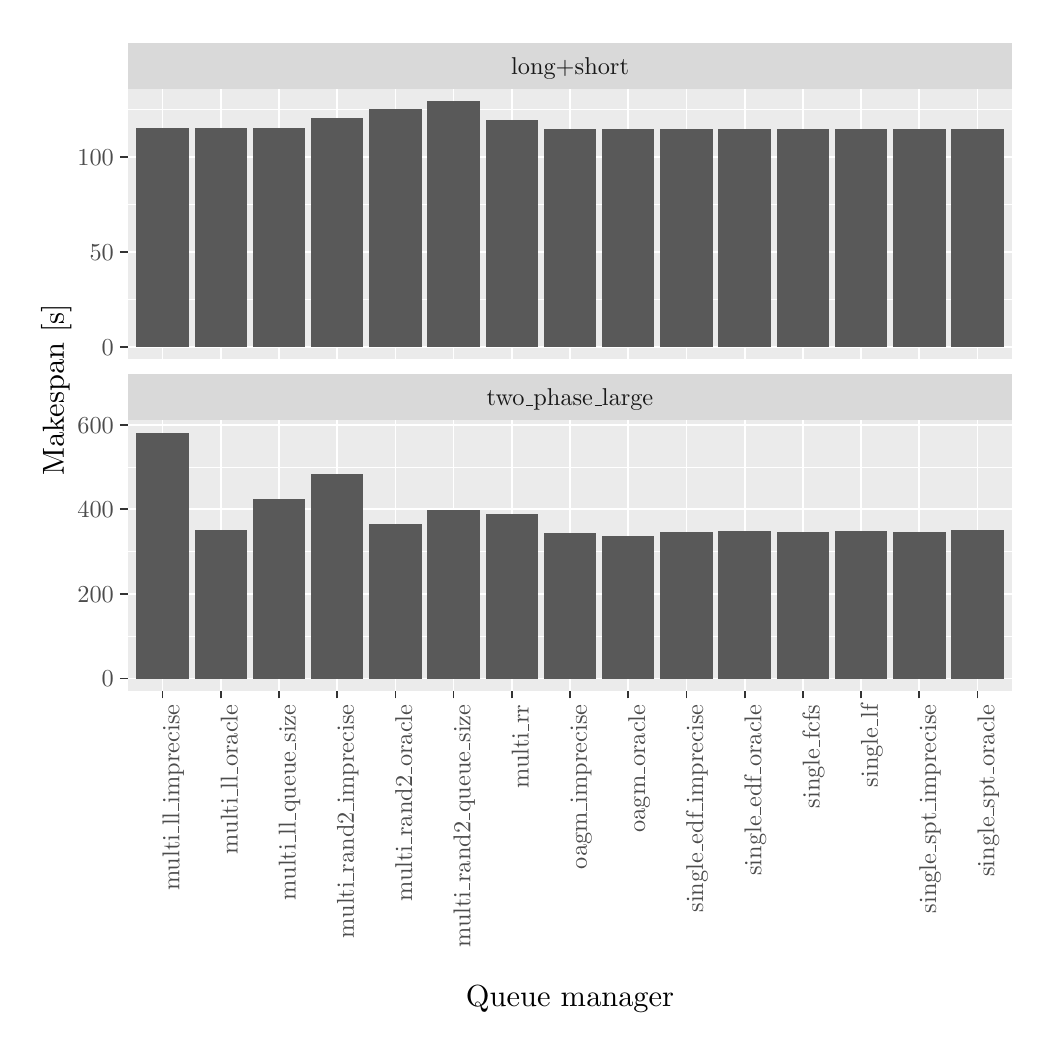
\begin{tikzpicture}[x=1pt,y=1pt]
\definecolor{fillColor}{RGB}{255,255,255}
\path[use as bounding box,fill=fillColor,fill opacity=0.00] (0,0) rectangle (361.35,361.35);
\begin{scope}
\path[clip] (  0.00,  0.00) rectangle (361.35,361.35);
\definecolor{drawColor}{RGB}{255,255,255}
\definecolor{fillColor}{RGB}{255,255,255}

\path[draw=drawColor,line width= 0.6pt,line join=round,line cap=round,fill=fillColor] (  0.00,  0.00) rectangle (361.35,361.35);
\end{scope}
\begin{scope}
\path[clip] ( 36.11,241.53) rectangle (355.85,339.28);
\definecolor{fillColor}{gray}{0.92}

\path[fill=fillColor] ( 36.11,241.53) rectangle (355.85,339.28);
\definecolor{drawColor}{RGB}{255,255,255}

\path[draw=drawColor,line width= 0.3pt,line join=round] ( 36.11,263.11) --
	(355.85,263.11);

\path[draw=drawColor,line width= 0.3pt,line join=round] ( 36.11,297.37) --
	(355.85,297.37);

\path[draw=drawColor,line width= 0.3pt,line join=round] ( 36.11,331.63) --
	(355.85,331.63);

\path[draw=drawColor,line width= 0.6pt,line join=round] ( 36.11,245.98) --
	(355.85,245.98);

\path[draw=drawColor,line width= 0.6pt,line join=round] ( 36.11,280.24) --
	(355.85,280.24);

\path[draw=drawColor,line width= 0.6pt,line join=round] ( 36.11,314.50) --
	(355.85,314.50);

\path[draw=drawColor,line width= 0.6pt,line join=round] ( 48.73,241.53) --
	( 48.73,339.28);

\path[draw=drawColor,line width= 0.6pt,line join=round] ( 69.77,241.53) --
	( 69.77,339.28);

\path[draw=drawColor,line width= 0.6pt,line join=round] ( 90.80,241.53) --
	( 90.80,339.28);

\path[draw=drawColor,line width= 0.6pt,line join=round] (111.84,241.53) --
	(111.84,339.28);

\path[draw=drawColor,line width= 0.6pt,line join=round] (132.87,241.53) --
	(132.87,339.28);

\path[draw=drawColor,line width= 0.6pt,line join=round] (153.91,241.53) --
	(153.91,339.28);

\path[draw=drawColor,line width= 0.6pt,line join=round] (174.95,241.53) --
	(174.95,339.28);

\path[draw=drawColor,line width= 0.6pt,line join=round] (195.98,241.53) --
	(195.98,339.28);

\path[draw=drawColor,line width= 0.6pt,line join=round] (217.02,241.53) --
	(217.02,339.28);

\path[draw=drawColor,line width= 0.6pt,line join=round] (238.05,241.53) --
	(238.05,339.28);

\path[draw=drawColor,line width= 0.6pt,line join=round] (259.09,241.53) --
	(259.09,339.28);

\path[draw=drawColor,line width= 0.6pt,line join=round] (280.12,241.53) --
	(280.12,339.28);

\path[draw=drawColor,line width= 0.6pt,line join=round] (301.16,241.53) --
	(301.16,339.28);

\path[draw=drawColor,line width= 0.6pt,line join=round] (322.19,241.53) --
	(322.19,339.28);

\path[draw=drawColor,line width= 0.6pt,line join=round] (343.23,241.53) --
	(343.23,339.28);
\definecolor{fillColor}{gray}{0.35}

\path[fill=fillColor] ( 39.27,245.98) rectangle ( 58.20,324.92);

\path[fill=fillColor] ( 60.30,245.98) rectangle ( 79.23,324.92);

\path[fill=fillColor] ( 81.34,245.98) rectangle (100.27,324.92);

\path[fill=fillColor] (102.37,245.98) rectangle (121.30,328.60);

\path[fill=fillColor] (123.41,245.98) rectangle (142.34,331.91);

\path[fill=fillColor] (144.44,245.98) rectangle (163.38,334.84);

\path[fill=fillColor] (165.48,245.98) rectangle (184.41,327.92);

\path[fill=fillColor] (186.51,245.98) rectangle (205.45,324.73);

\path[fill=fillColor] (207.55,245.98) rectangle (226.48,324.73);

\path[fill=fillColor] (228.59,245.98) rectangle (247.52,324.73);

\path[fill=fillColor] (249.62,245.98) rectangle (268.55,324.73);

\path[fill=fillColor] (270.66,245.98) rectangle (289.59,324.73);

\path[fill=fillColor] (291.69,245.98) rectangle (310.62,324.73);

\path[fill=fillColor] (312.73,245.98) rectangle (331.66,324.73);

\path[fill=fillColor] (333.76,245.98) rectangle (352.69,324.73);
\end{scope}
\begin{scope}
\path[clip] ( 36.11,121.72) rectangle (355.85,219.46);
\definecolor{fillColor}{gray}{0.92}

\path[fill=fillColor] ( 36.11,121.72) rectangle (355.85,219.46);
\definecolor{drawColor}{RGB}{255,255,255}

\path[draw=drawColor,line width= 0.3pt,line join=round] ( 36.11,141.45) --
	(355.85,141.45);

\path[draw=drawColor,line width= 0.3pt,line join=round] ( 36.11,172.02) --
	(355.85,172.02);

\path[draw=drawColor,line width= 0.3pt,line join=round] ( 36.11,202.60) --
	(355.85,202.60);

\path[draw=drawColor,line width= 0.6pt,line join=round] ( 36.11,126.16) --
	(355.85,126.16);

\path[draw=drawColor,line width= 0.6pt,line join=round] ( 36.11,156.74) --
	(355.85,156.74);

\path[draw=drawColor,line width= 0.6pt,line join=round] ( 36.11,187.31) --
	(355.85,187.31);

\path[draw=drawColor,line width= 0.6pt,line join=round] ( 36.11,217.89) --
	(355.85,217.89);

\path[draw=drawColor,line width= 0.6pt,line join=round] ( 48.73,121.72) --
	( 48.73,219.46);

\path[draw=drawColor,line width= 0.6pt,line join=round] ( 69.77,121.72) --
	( 69.77,219.46);

\path[draw=drawColor,line width= 0.6pt,line join=round] ( 90.80,121.72) --
	( 90.80,219.46);

\path[draw=drawColor,line width= 0.6pt,line join=round] (111.84,121.72) --
	(111.84,219.46);

\path[draw=drawColor,line width= 0.6pt,line join=round] (132.87,121.72) --
	(132.87,219.46);

\path[draw=drawColor,line width= 0.6pt,line join=round] (153.91,121.72) --
	(153.91,219.46);

\path[draw=drawColor,line width= 0.6pt,line join=round] (174.95,121.72) --
	(174.95,219.46);

\path[draw=drawColor,line width= 0.6pt,line join=round] (195.98,121.72) --
	(195.98,219.46);

\path[draw=drawColor,line width= 0.6pt,line join=round] (217.02,121.72) --
	(217.02,219.46);

\path[draw=drawColor,line width= 0.6pt,line join=round] (238.05,121.72) --
	(238.05,219.46);

\path[draw=drawColor,line width= 0.6pt,line join=round] (259.09,121.72) --
	(259.09,219.46);

\path[draw=drawColor,line width= 0.6pt,line join=round] (280.12,121.72) --
	(280.12,219.46);

\path[draw=drawColor,line width= 0.6pt,line join=round] (301.16,121.72) --
	(301.16,219.46);

\path[draw=drawColor,line width= 0.6pt,line join=round] (322.19,121.72) --
	(322.19,219.46);

\path[draw=drawColor,line width= 0.6pt,line join=round] (343.23,121.72) --
	(343.23,219.46);
\definecolor{fillColor}{gray}{0.35}

\path[fill=fillColor] ( 39.27,126.16) rectangle ( 58.20,215.02);

\path[fill=fillColor] ( 60.30,126.16) rectangle ( 79.23,179.69);

\path[fill=fillColor] ( 81.34,126.16) rectangle (100.27,191.12);

\path[fill=fillColor] (102.37,126.16) rectangle (121.30,199.91);

\path[fill=fillColor] (123.41,126.16) rectangle (142.34,181.85);

\path[fill=fillColor] (144.44,126.16) rectangle (163.38,187.19);

\path[fill=fillColor] (165.48,126.16) rectangle (184.41,185.75);

\path[fill=fillColor] (186.51,126.16) rectangle (205.45,178.69);

\path[fill=fillColor] (207.55,126.16) rectangle (226.48,177.84);

\path[fill=fillColor] (228.59,126.16) rectangle (247.52,179.26);

\path[fill=fillColor] (249.62,126.16) rectangle (268.55,179.57);

\path[fill=fillColor] (270.66,126.16) rectangle (289.59,179.01);

\path[fill=fillColor] (291.69,126.16) rectangle (310.62,179.39);

\path[fill=fillColor] (312.73,126.16) rectangle (331.66,179.14);

\path[fill=fillColor] (333.76,126.16) rectangle (352.69,179.71);
\end{scope}
\begin{scope}
\path[clip] ( 36.11,219.46) rectangle (355.85,236.03);
\definecolor{fillColor}{gray}{0.85}

\path[fill=fillColor] ( 36.11,219.46) rectangle (355.85,236.03);
\definecolor{drawColor}{gray}{0.10}

\node[text=drawColor,anchor=base,inner sep=0pt, outer sep=0pt, scale=  0.88] at (195.98,224.72) {two\_phase\_large};
\end{scope}
\begin{scope}
\path[clip] ( 36.11,339.28) rectangle (355.85,355.85);
\definecolor{fillColor}{gray}{0.85}

\path[fill=fillColor] ( 36.11,339.28) rectangle (355.85,355.85);
\definecolor{drawColor}{gray}{0.10}

\node[text=drawColor,anchor=base,inner sep=0pt, outer sep=0pt, scale=  0.88] at (195.98,344.53) {long+short};
\end{scope}
\begin{scope}
\path[clip] (  0.00,  0.00) rectangle (361.35,361.35);
\definecolor{drawColor}{gray}{0.20}

\path[draw=drawColor,line width= 0.6pt,line join=round] ( 48.73,118.97) --
	( 48.73,121.72);

\path[draw=drawColor,line width= 0.6pt,line join=round] ( 69.77,118.97) --
	( 69.77,121.72);

\path[draw=drawColor,line width= 0.6pt,line join=round] ( 90.80,118.97) --
	( 90.80,121.72);

\path[draw=drawColor,line width= 0.6pt,line join=round] (111.84,118.97) --
	(111.84,121.72);

\path[draw=drawColor,line width= 0.6pt,line join=round] (132.87,118.97) --
	(132.87,121.72);

\path[draw=drawColor,line width= 0.6pt,line join=round] (153.91,118.97) --
	(153.91,121.72);

\path[draw=drawColor,line width= 0.6pt,line join=round] (174.95,118.97) --
	(174.95,121.72);

\path[draw=drawColor,line width= 0.6pt,line join=round] (195.98,118.97) --
	(195.98,121.72);

\path[draw=drawColor,line width= 0.6pt,line join=round] (217.02,118.97) --
	(217.02,121.72);

\path[draw=drawColor,line width= 0.6pt,line join=round] (238.05,118.97) --
	(238.05,121.72);

\path[draw=drawColor,line width= 0.6pt,line join=round] (259.09,118.97) --
	(259.09,121.72);

\path[draw=drawColor,line width= 0.6pt,line join=round] (280.12,118.97) --
	(280.12,121.72);

\path[draw=drawColor,line width= 0.6pt,line join=round] (301.16,118.97) --
	(301.16,121.72);

\path[draw=drawColor,line width= 0.6pt,line join=round] (322.19,118.97) --
	(322.19,121.72);

\path[draw=drawColor,line width= 0.6pt,line join=round] (343.23,118.97) --
	(343.23,121.72);
\end{scope}
\begin{scope}
\path[clip] (  0.00,  0.00) rectangle (361.35,361.35);
\definecolor{drawColor}{gray}{0.30}

\node[text=drawColor,rotate= 90.00,anchor=base east,inner sep=0pt, outer sep=0pt, scale=  0.88] at ( 54.79,116.77) {multi\_ll\_imprecise};

\node[text=drawColor,rotate= 90.00,anchor=base east,inner sep=0pt, outer sep=0pt, scale=  0.88] at ( 75.83,116.77) {multi\_ll\_oracle};

\node[text=drawColor,rotate= 90.00,anchor=base east,inner sep=0pt, outer sep=0pt, scale=  0.88] at ( 96.86,116.77) {multi\_ll\_queue\_size};

\node[text=drawColor,rotate= 90.00,anchor=base east,inner sep=0pt, outer sep=0pt, scale=  0.88] at (117.90,116.77) {multi\_rand2\_imprecise};

\node[text=drawColor,rotate= 90.00,anchor=base east,inner sep=0pt, outer sep=0pt, scale=  0.88] at (138.94,116.77) {multi\_rand2\_oracle};

\node[text=drawColor,rotate= 90.00,anchor=base east,inner sep=0pt, outer sep=0pt, scale=  0.88] at (159.97,116.77) {multi\_rand2\_queue\_size};

\node[text=drawColor,rotate= 90.00,anchor=base east,inner sep=0pt, outer sep=0pt, scale=  0.88] at (181.01,116.77) {multi\_rr};

\node[text=drawColor,rotate= 90.00,anchor=base east,inner sep=0pt, outer sep=0pt, scale=  0.88] at (202.04,116.77) {oagm\_imprecise};

\node[text=drawColor,rotate= 90.00,anchor=base east,inner sep=0pt, outer sep=0pt, scale=  0.88] at (223.08,116.77) {oagm\_oracle};

\node[text=drawColor,rotate= 90.00,anchor=base east,inner sep=0pt, outer sep=0pt, scale=  0.88] at (244.11,116.77) {single\_edf\_imprecise};

\node[text=drawColor,rotate= 90.00,anchor=base east,inner sep=0pt, outer sep=0pt, scale=  0.88] at (265.15,116.77) {single\_edf\_oracle};

\node[text=drawColor,rotate= 90.00,anchor=base east,inner sep=0pt, outer sep=0pt, scale=  0.88] at (286.18,116.77) {single\_fcfs};

\node[text=drawColor,rotate= 90.00,anchor=base east,inner sep=0pt, outer sep=0pt, scale=  0.88] at (307.22,116.77) {single\_lf};

\node[text=drawColor,rotate= 90.00,anchor=base east,inner sep=0pt, outer sep=0pt, scale=  0.88] at (328.25,116.77) {single\_spt\_imprecise};

\node[text=drawColor,rotate= 90.00,anchor=base east,inner sep=0pt, outer sep=0pt, scale=  0.88] at (349.29,116.77) {single\_spt\_oracle};
\end{scope}
\begin{scope}
\path[clip] (  0.00,  0.00) rectangle (361.35,361.35);
\definecolor{drawColor}{gray}{0.30}

\node[text=drawColor,anchor=base east,inner sep=0pt, outer sep=0pt, scale=  0.88] at ( 31.16,242.95) {0};

\node[text=drawColor,anchor=base east,inner sep=0pt, outer sep=0pt, scale=  0.88] at ( 31.16,277.21) {50};

\node[text=drawColor,anchor=base east,inner sep=0pt, outer sep=0pt, scale=  0.88] at ( 31.16,311.47) {100};
\end{scope}
\begin{scope}
\path[clip] (  0.00,  0.00) rectangle (361.35,361.35);
\definecolor{drawColor}{gray}{0.20}

\path[draw=drawColor,line width= 0.6pt,line join=round] ( 33.36,245.98) --
	( 36.11,245.98);

\path[draw=drawColor,line width= 0.6pt,line join=round] ( 33.36,280.24) --
	( 36.11,280.24);

\path[draw=drawColor,line width= 0.6pt,line join=round] ( 33.36,314.50) --
	( 36.11,314.50);
\end{scope}
\begin{scope}
\path[clip] (  0.00,  0.00) rectangle (361.35,361.35);
\definecolor{drawColor}{gray}{0.30}

\node[text=drawColor,anchor=base east,inner sep=0pt, outer sep=0pt, scale=  0.88] at ( 31.16,123.13) {0};

\node[text=drawColor,anchor=base east,inner sep=0pt, outer sep=0pt, scale=  0.88] at ( 31.16,153.71) {200};

\node[text=drawColor,anchor=base east,inner sep=0pt, outer sep=0pt, scale=  0.88] at ( 31.16,184.28) {400};

\node[text=drawColor,anchor=base east,inner sep=0pt, outer sep=0pt, scale=  0.88] at ( 31.16,214.85) {600};
\end{scope}
\begin{scope}
\path[clip] (  0.00,  0.00) rectangle (361.35,361.35);
\definecolor{drawColor}{gray}{0.20}

\path[draw=drawColor,line width= 0.6pt,line join=round] ( 33.36,126.16) --
	( 36.11,126.16);

\path[draw=drawColor,line width= 0.6pt,line join=round] ( 33.36,156.74) --
	( 36.11,156.74);

\path[draw=drawColor,line width= 0.6pt,line join=round] ( 33.36,187.31) --
	( 36.11,187.31);

\path[draw=drawColor,line width= 0.6pt,line join=round] ( 33.36,217.89) --
	( 36.11,217.89);
\end{scope}
\begin{scope}
\path[clip] (  0.00,  0.00) rectangle (361.35,361.35);
\definecolor{drawColor}{RGB}{0,0,0}

\node[text=drawColor,anchor=base,inner sep=0pt, outer sep=0pt, scale=  1.10] at (195.98,  7.64) {Queue manager};
\end{scope}
\begin{scope}
\path[clip] (  0.00,  0.00) rectangle (361.35,361.35);
\definecolor{drawColor}{RGB}{0,0,0}

\node[text=drawColor,rotate= 90.00,anchor=base,inner sep=0pt, outer sep=0pt, scale=  1.10] at ( 13.08,230.50) {Makespan [s]};
\end{scope}
\end{tikzpicture}
